\documentclass[12pt]{article}

\input preamble

\title{Principles of Parallel Architecture\\
Project Report 3}
\author{Xitong Liu \\
xliu@ece.udel.edu}

\begin{document}

\maketitle

\section{Introduction}
In this report, we will introduce the methods applied to optimize
the performance of Matrix Multiplication on parallel architecture.
Results showed that the performance has been improved a lot comparing
to the baseline approach proposed in the previous report.


\section{Experiment Results}
\subsection{Experiment Setup}
The matrix size is $1024\times 1024$ in float numbers and number of 
threads is 32. We apply different optimization methods step by step, 
and new optimization method is combined with the previous one. Since 
it's limited by the space, we assign different method combinations to 
different IDs, shown in Table~\ref{tab:methods}.

\begin{table}[h!]
	\small
	\begin{center}
	\caption{\label{tab:methods} Method Combinations ID Map}
	\begin{tabular}{|r|l|}
		\hline
		ID & Method Combination \\ \hline
		0 &	Serial \\ \hline
		1 & Baseline \\ \hline
    2 & Transpose \\ \hline
    3 & Transpose + SSE \\ \hline
    4 & Transpose + SSE + Unrolling (4 cycles) + Scheduling \\ \hline
    5 & Transpose + SSE + Unrolling (2 cycles) + Scheduling + 
      Software pipelining \\ \hline
	\end{tabular}
	\end{center}
\end{table}

\subsection{Results}
To explore the performances under different optimization settings by 
the compiler, we run the experiments in two groups: one with 
\texttt{-O3} option and the other without any optimization. For 
each setup, we run the program 20 times and calculate the average 
run time as the measurement of performance. The results are shown in 
Table~\ref{tab:performance}.

\begin{table}[h!]
	\small
	\begin{center}
	\caption{\label{tab:performance} Performance Comparison}
	\begin{tabular}{|r|r|r|r|r|}
		\hline
		 & \multicolumn{2}{c|}{NO Optimization} & \multicolumn{2}{c|}{-O3 Optimization} \\ \hline
		Method & Time(s) & Speed Up & Time(s) & Speed Up \\ \hline
		0  &  33.7776	& 1.0000		&19.4682		&	1.0000 \\ \hline
		1  &		4.5976		&	7.3468		& 2.3256		&	8.3712 \\ \hline
		2  &		4.1109  & 8.2166		&	0.4622		&	42.1209 \\ \hline
		3  &		0.9353  & 36.1142	&	0.4656		&	41.8133 \\ \hline
		4  &		0.6091  & \textbf{55.4550}	& 0.4208		&	\textbf {46.2649} \\ \hline
		5  &		0.7761  & 43.5223	&	0.4660		&	41.7774 \\ \hline
	\end{tabular}
	\end{center}
\end{table}

\subsection{Analysis}
Based on the observations in the results, we can draw the following interesting 
conclusions:
\begin{enumerate}
\item Our current best performance (Method 4) without any optimization has reached 
the 60\% of the best performance with -O3 optimization.
\end{enumerate}

\section{Conclusion}

\end{document}

\begin{comment}
\begin{figure}[h!]
	\begin{center}
		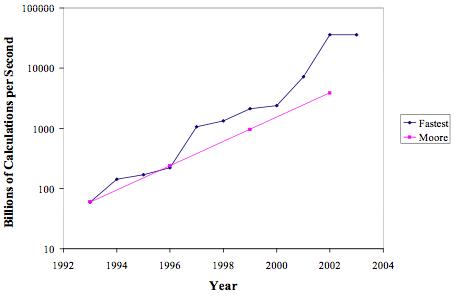
\includegraphics[width=0.7\textwidth, angle=0]{fatest.png}
		\caption{\label{fig:fatest}Fatest SuperComputer in the world}
	\end{center}
\end{figure}
\end{comment}